%
\section{File transfer protocols}
\label{sec:file-transf-prot}
Sometimes during the operation of all the system, it is necessary to transfer file between machines, for example, when a brand wants to upload video advertisements to its rent, or even when the admin wants to download that ad to verify its reliability.

\subsection{Protocols Overview}
\label{sub-sec:prot-overview}

There are various file transfer protocols to use, with different features and types of security and reliability. Throughout this various protocols, these are the most common ones~\cite{file-transf-protoc}:
%
\begin{item-c}
\item \emph{FTP}: it is a popular file transfer method that has been around for decades. FTP exchanges data using two separate channels known as the \texttt{command channel} to authenticate the user, and the \texttt{data channel} to transfer the files.
With FTP, both channels are \texttt{unencrypted}, leaving any data sent over these channels vulnerable to being taken advantage of. However, it does require an authenticated username and password for access.
%
\item \emph{FTPS}: it is a secure file transfer protocol that allows you to transfer files securely with trading partners, customers, and users. The transfers can be authenticated through FTPS-supported methods like client certificates, server certificates, and passwords.
%
\item \emph{SFTP}: it is a secure FTP protocol and a great alternative to unsecure FTP tools or manual scripts. SFTP exchanges data over an SSH connection and provides organizations with a high level of protection for file transfers shared between their systems, trading partners, employees, and the cloud.
%
\item \emph{SCP}: it is a network protocol that supports file transfers between hosts on a computer network. It's somewhat similar to FTP, however, SCP supports encryption and authentication features.
%
\item \emph{HTTP}: it is the foundation of data communication. It defines the format of messages through which web browsers and web servers communicate and defines how a web browser should response to a web request. HTTP uses \gls{tcp} as an underlying transport and is a stateless protocol. This means each command is executed independently and no session information is retained by the receiver.
%
\item \emph{HTTPS}: it is the secure version of HTTP where communications are encrypted by TLS or SSL.
\end{item-c}

\subsection{Which protocol is more efficient?}
\label{sub-sec:prot-effic}

In this case, \texttt{security} is one of the main goals, which means that all data must be sent in the best secure way possible. Thus, all file transfers must have \texttt{authentications} and \texttt{encryption}.
%
In conclusion, the better choice to this system is to chose the \texttt{HTTPS} protocol for several reasons:
\begin{item-c}
\item The communications between subsystems are made through \gls{tcp}/\gls{ip}, this is also used in this protocol, which is an advantage;
\item The data is transferred only with authentications (request and responses) which makes it more secure;
\item all communication is encrypted, which makes it even more secure.
\end{item-c} 

\subsection{Example of how to transfer files}
\label{sub-sec:file-transf-ex}

Here are examples on how to configure a connection fot file transfers and also how to download a file from a remote server using HTTPS.

\subsubsection{Configuring HTTP Connection Characteristics for File Transfers}
The following task is used to customize the connection characteristics for your network to specify a username and password, connection preferences, a remote proxy server, and the source interface to be used. These are the summary steps (that are then explained on Fig.~\ref{fig:configure-http-1} and Fig.~\ref{fig:configure-http-2})~\cite{http-example-cisco}:
%
\begin{enum-c}
\item enable;
\item configure terminal;
\item ip http client connection {forceclose | idletimeout <\texttt{seconds}> | timeout <\texttt{seconds}>};
\item ip http client username <\texttt{username}>;
\item ip http client password <\texttt{password}>;
\item ip http client proxy-server {<\texttt{proxy-name}> | <\texttt{ip-address}} [proxy-port <\texttt{port-number}>];
\item ip http client source-interface <\texttt{interface-id}>;
\item do copy running-config startup-config;
\item end.
\end{enum-c}
%
\begin{figure}[!hbt]
\centering
    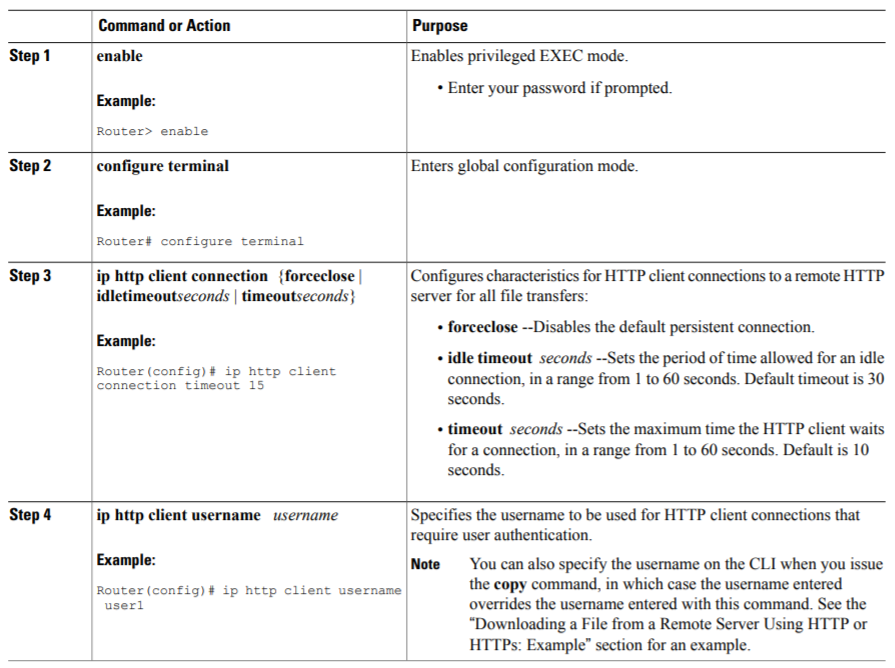
\includegraphics[width=0.8\textwidth]{./img/configure-http-1.png}
  \caption{Configuring HTTP Connection - 1(withdrawn from~\cite{http-example-cisco})}%
\label{fig:configure-http-1}
\end{figure}
%
\begin{figure}[!hbt]
\centering
    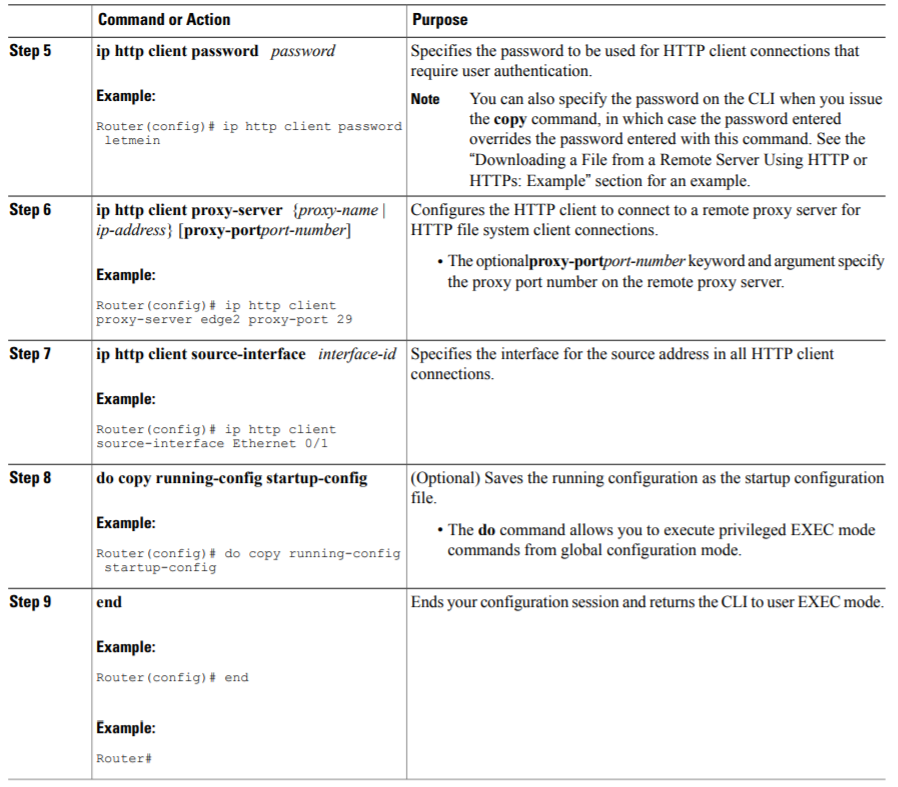
\includegraphics[width=0.8\textwidth]{./img/configure-http-2.png}
  \caption{Configuring HTTP Connection - 2(withdrawn from~\cite{http-example-cisco})}%
\label{fig:configure-http-2}
\end{figure}
%
\subsubsection{Downloading a File from a Remote Server Using HTTP or HTTPS}
Perform this task to download a file from a remote HTTP server using HTTP or HTTPs. The copy command helps you to copy any file from a source to a destination. These are the summary steps (that are then explained on Fig.~\ref{fig:download-http-1} and Fig.~\ref{fig:download-http-2})~\cite{http-example-cisco}:
%
\begin{enum-c}
\item enable;
\item Do one of the following:
	\begin{item-c}
	\item copy [/erase] [/noverify] http://<\texttt{remote-source-urllocal-destination-url}>;
	\item copy https:// <\texttt{remote-source-url local-destination-url}>.
	\end{item-c}
\end{enum-c}
%
\begin{figure}[!hbt]
\centering
    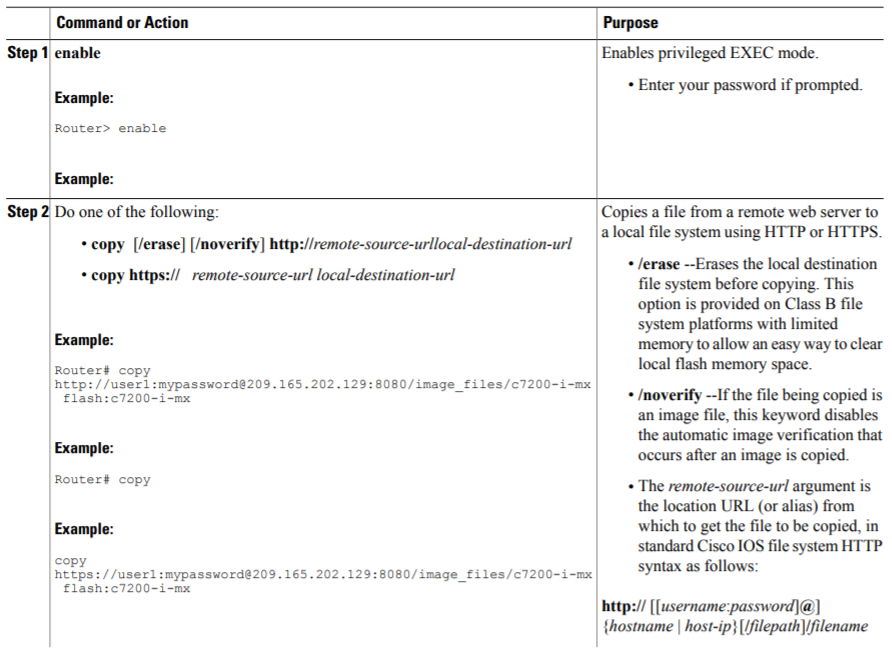
\includegraphics[width=0.8\textwidth]{./img/download-http-1.png}
  \caption{Downloading a File using HTTP - 1(withdrawn from~\cite{http-example-cisco})}%
\label{fig:download-http-1}
\end{figure}
%
\begin{figure}[!hbt]
\centering
    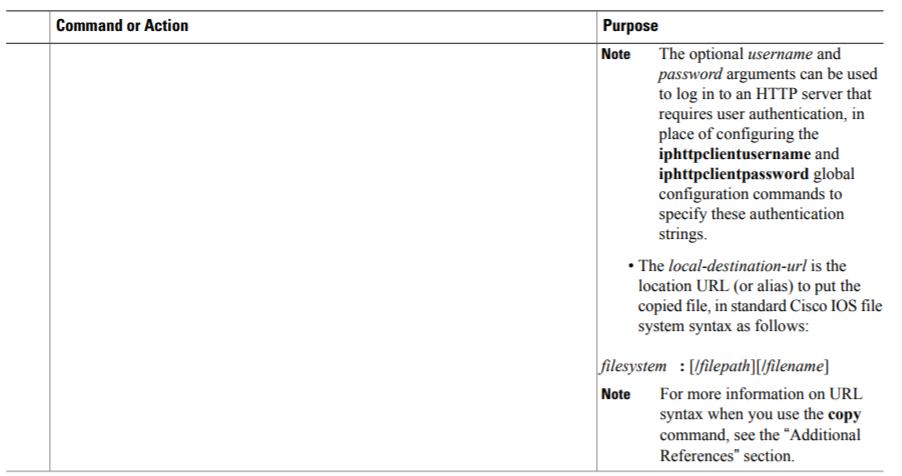
\includegraphics[width=0.8\textwidth]{./img/download-http-2.png}
  \caption{Downloading a File using HTTP - 2(withdrawn from~\cite{http-example-cisco})}%
\label{fig:download-http-2}
\end{figure}

\subsection{File Transfer Protocol \gls{api}s}
\label{sub-sec:ftp-apis}
There are several \gls{api}s that allow to develop applications in order to transfer files between two distinct points using file transfer protocols. The most common is \texttt{libcurl}, however, this is used in C language and it is necessary to use a wrapper to follow \gls{oop} paradigm, as it was previously said on subsection \ref{sec:c++-libraries-apis}.

In this case, it will be used one of the wrappers previously mentioned \texttt{curlpp}.

In Listing \ref{lst:http-post-ex} is an example on how does an HTTP POST is done. Basically it is crated an \texttt{easy} object that will handle all the POST request, inserting the \gls{url}, the header and the POST's field and size, then it is just needed to perform the request.
%
\lstinputlisting[language=C++, firstline=1,
caption={POST example using <curlpp.h>},
label=lst:http-post-ex,
style= custom-cpp]{./listing/http-post-ex.cpp}

\subsubsection{Third-party applications}

To make the file transfer more easier, it will be used a third-party application named \texttt{transfer.sh}. This application has easy-to-use commands in order to transfer files with a \gls{url}, there is unlimited upload, it can encrypt files and it is also possible to limit the amount of downloads and days available of downloading~\cite{transfer-sh}.

With a simple command like \texttt{curl --upload-file <path-to-the-file> https://transfer.sh/<name-that-you-want>} the file is uploaded to the site and it generates a \gls{url} to transfer that file using the command \texttt{curl <generated-url> -o <name-you-want>}.
And with this simple steps it is possible to easily transfer files between two nodes.

Using the library \texttt{curlpp} with the \texttt{transfer.sh} \gls{api}, it is possible to create a program to transfer files between nodes automatically when requested from the user, without the user needs to decorate or do such commands.
%
%%% Local Variables:
%%% mode: latex
%%% TeX-master: "../../../dissertation"
%%% End:
